\documentclass[11pt,a4paper]{article}
\usepackage[margin=2.6cm]{geometry}
\usepackage[T1]{fontenc}
\usepackage{lmodern}
\usepackage{amsmath,amssymb,amsthm}
\usepackage{graphicx}
\usepackage{booktabs}
\usepackage{enumitem}
\usepackage[hidelinks]{hyperref}
\usepackage{caption}
\usepackage{float}
\usepackage{cite}
\captionsetup{font=small,labelfont=bf}
\setlength{\parskip}{0.55em}
\setlength{\parindent}{0pt}
\setlist{itemsep=0.15em,topsep=0.3em}

\theoremstyle{definition}
\newtheorem{definition}{Definition}
\newtheorem{assumption}{Assumption}
\newtheorem{remark}{Remark}
\newtheorem{observation}{Observation}
\theoremstyle{plain}
\newtheorem{lemma}{Lemma}
\newtheorem{proposition}{Proposition}
\newtheorem{corollary}{Corollary}
\newtheorem{conjecture}{Conjecture}

\newcommand{\Binf}{B}
\newcommand{\xs}{x^{*}}
\newcommand{\KL}{\mathrm{KL}}
\newcommand{\En}{\mathcal{E}}

\title{\textbf{The smallest steering budget for\\ exponential-weights learners in a coordination game}\\[0.4em]
\large The energy identity read as a cost, and the role of the interaction graph}
\author{Aditya Maiti}
\date{22 November 2026}

\pdfinfoomitdate=1
\pdfsuppressptexinfo=-1
\pdftrailerid{}
\newcommand{\codeurl}{github.com/ADITYA-WORK-MAITI/steering-budget}
\hypersetup{pdftitle={The smallest steering budget for exponential-weights learners in a coordination game},pdfauthor={Aditya Maiti}}
\begin{document}
\maketitle

\begin{abstract}
\noindent
Learners in a coordination game can settle at the inferior strict equilibrium and stay there.
A mediator can pay them to move.
Zhang et al.~\cite{zhang2024} ask for which learning dynamics a finite total budget is enough.
Huang et al.~\cite{huang2025} note that budget constraints could be added to their steering model.
This note computes the smallest budget in one case. The learners follow natural policy gradient with exact payoffs. In a normal-form game this is the exponential-weights rule. The game is a two-action coordination game on a graph. The payments and their cost are those of~\cite{huang2025}.

The tool is not new. It is the energy identity of exponential weights. Read with the unpaid action as base point, it splits the mediator's expected payment into three parts. The first is the rise of the Kullback--Leibler divergence from that action. The second is the learner's regret against that action in the game. The third, with a minus sign, is a Kullback--Leibler term from the finite step.

The results are for the small-step limit. A cost in this note is the total payment multiplied by the step size.
\begin{enumerate}
\item On the complete graph the infimum of the budget is $N\log\frac{1-x_0}{1-\xs}$, where $\xs$ is the mixed equilibrium and $x_0$ the common start. This is the rise of the Kullback--Leibler divergence from the inferior equilibrium between the start and the mixed equilibrium.
\item On the ring the budget changes regime near the contagion threshold $\tfrac12$ of Ellison and Morris. If $\xs<\tfrac12$ it lies between two constants that do not depend on $N$. If $\xs>\tfrac{1+x_0}{2}$ it is at least $\lceil N/2\rceil\log\frac{1-x_0}{2(1-\xs)}$.
\item The bounded budget on the ring costs time. If the mediator pays only at the start, the change spreads more and more slowly: each further agent takes $1/(1-2\xs)$ times longer than the one before. Very small holding payments remove the slowdown: the time is then at most of order $N\log N$. In simulations a small decay of the logits also removes it.
\item The two-player Stag Hunt experiment of~\cite{huang2025} is consistent with the identity. A simple threshold rule gives a curve of cost against the steering gap at the end of the horizon. With the payment charged as in their code, the three costs in their Figure~5 lie within about $0.4$ of this curve, which is the size of their error bars.
\end{enumerate}
Statements 1 and 2 and the holding-payment part of 3 are proved. The rest is numerical. Section~\ref{sec:new} says which parts are known. Section~\ref{sec:limits} says what the note does not show.
\end{abstract}

%=====================================================================
\section{Introduction}\label{sec:intro}

\paragraph{The question.}
Strict Nash equilibria are stable and attracting under regularised learning~\cite{giannou2021,mertikopoulos2023}. A coordination game has two strict equilibria. Learners that reach the inferior one stay there. Results on convergence say where learning ends. This note asks what it costs an outside party to change where it ends.

Two papers pose the question. Zhang et al.~\cite{zhang2024} show that no fixed total budget steers arbitrary no-regret learners (their Proposition~3.2, proved on a coordination game). Their conclusion asks for ``the class of learning dynamics under which the steering problem can be solved with a finite cumulative budget''. Huang et al.~\cite{huang2025} prove that a steering strategy exists for natural-policy-gradient learners when the horizon and the payment cap are large enough (their Theorem~4.2). They do not bound the cost of such a strategy. They write that ``constraints on the steering reward budget could be added''. A budget constraint can be met only above the smallest possible cost. This note computes that cost for one learning rule and one class of games.

\paragraph{Scope.}
The agents follow natural policy gradient with exact advantages, the rule of the Stag Hunt experiment in~\cite{huang2025}. In a normal-form game this is the exponential-weights rule. The game is a two-action coordination game played with neighbours on a graph. The mediator pays non-negative rewards that depend on the agent's action, and its cost is the expected payment. Two graphs are treated: the complete graph and the ring.

\paragraph{The objective differs from that of Huang et al.}
Huang et al.\ fix a horizon $T$ and minimise the steering gap at the end, with the cost as a second goal. The steering gap is the largest possible total utility minus the total utility of the policies. I call its value at the end of the horizon the terminal gap. I ask a different question: what is the smallest cost of entering the basin of the better equilibrium, with no deadline? The two costs differ a lot. In their two-player experiment the rescaled horizon is $\alpha T=5$. From $(0.1,0.1)$, one of the $25$ starts of that experiment, the smallest cost of entering the basin is $1.99$ (about $2.10$ with symmetric payments at their cap and step size, Table~\ref{tab:steps}). Reaching the three terminal gaps they report costs between $7.1$ and $10.6$ from that start with the threshold rule of Section~\ref{sec:bench}. The difference pays for coming that close to all-$H$ within the horizon. On the ring the strategies that are cheaper than the symmetric one are slow. In the runs of Section~\ref{sec:fronts} they take a rescaled time from about $20$ to more than $10^4$.

\paragraph{Known and new parts.}\label{sec:new}
\begin{itemize}
\item The identity of Lemma~\ref{lem:identity} is standard. Remark~\ref{rem:origin} gives its sources. What I add is its reading as the mediator's cost.
\item The value $N\log\frac{1-x_0}{1-\xs}$ follows from the identity and Jensen's inequality. I did not find it stated.
\item The threshold $\tfrac12$ on the ring is the contagion threshold of Ellison, as presented by \mbox{Morris}~\cite{morris2000}. For threshold agents on a path, incentive costs with the same split are known~\cite{cordasco2018} (Section~\ref{sec:ring}). Propositions~\ref{prop:ring-low} and~\ref{prop:ring-high} are the counterpart for learners with mixed policies and expected-payment cost.
\item The slowdown ratio $1/(1-2\xs)$ is a numerical observation with a short derivation. I did not find it stated. Its mechanism is related to the lower bounds of Panageas et al.~\cite{panageas2023} for fictitious play and of Anagnostides et al.~\cite{anagnostides2026} for follow-the-regularised-leader (Section~\ref{sec:time}).
\item Proposition~\ref{prop:hold} on holding payments and the comparison with Figure~5 of~\cite{huang2025} are small. I did not find them stated.
\end{itemize}
My search for earlier statements was limited to open sources. I may have missed some.

An earlier report of mine~\cite{maiti2026} treated a different game on the complete graph and on rings. There the number of attractors fell with the population size on the complete graph and grew on the ring. This is why the two graphs are compared here.

%=====================================================================
\section{Setting}\label{sec:setting}

\begin{definition}[Coordination game on a graph]\label{def:game}
There are $N$ agents. Agent $i$ has a non-empty set of neighbours $\mathcal N_i$. Each agent has two actions, $H$ and $G$. A pair of neighbours plays the symmetric game with payoffs $R$ for $(H,H)$, $S$ for $H$ against $G$, $T$ for $G$ against $H$, and $P$ for $(G,G)$, with $R>T$ and $P>S$. The reward of an agent is the average payoff over its neighbours. I also take $R>P$, so that all-$H$ is the better equilibrium; the mathematics does not use this. Define
\[
c=(R-T)+(P-S)>0,\qquad \xs=\frac{P-S}{c}\in(0,1).
\]
\end{definition}

Write $x_i\in(0,1)$ for the probability that agent $i$ plays $H$ and $m_i=\frac{1}{|\mathcal N_i|}\sum_{j\in\mathcal N_i}x_j$ for the average over its neighbours. The expected reward of $H$ minus that of $G$ for agent $i$ is
\begin{equation}\label{eq:g}
g_i(x)=c\,(m_i-\xs).
\end{equation}
Both all-$H$ and all-$G$ are strict equilibria. The symmetric mixed equilibrium is $x_i=\xs$ for all $i$. For the Stag Hunt of~\cite{huang2025}, $(R,S,T,P)=(5,0,4,2)$, so $c=3$ and $\xs=\tfrac23$.

On the \emph{complete graph} $\mathcal N_i$ is everyone except $i$. On the \emph{ring} $\mathcal N_i=\{i-1,i+1\}$ modulo $N$, with $N\ge3$. The unsteered dynamics are a replicator equation on a network, of the kind introduced by Madeo and Mocenni~\cite{madeo2015}.

\begin{remark}[Risk dominance and the potential]\label{rem:risk}
The action $H$ is strictly risk dominant when $R-T>P-S$, that is, when $\xs<\tfrac12$. On a connected regular graph the game is a potential game. The pair potential is $R-T$ at $(H,H)$, $P-S$ at $(G,G)$ and $0$ otherwise, and all-$H$ is the unique maximiser of the potential exactly when $\xs<\tfrac12$. In the Stag Hunt of~\cite{huang2025} the target $H$ is not risk dominant.
\end{remark}

\begin{definition}[Steered learning]\label{def:npg}
Let $\theta_i=\log\frac{x_i}{1-x_i}$ be the logit of agent $i$. In step $t$ the mediator offers agent $i$ the rewards $u_i^t(H),u_i^t(G)\in[0,U_{\max}]$. Write $v_i^t=u_i^t(H)-u_i^t(G)$. Natural policy gradient with step size $\alpha$ and exact advantages (Definition~4.1 of~\cite{huang2025}; see also~\cite{kakade2001,agarwal2021}) gives
\begin{equation}\label{eq:update}
\theta_i^{t+1}=\theta_i^{t}+\alpha\bigl(g_i(x^t)+v_i^t\bigr).
\end{equation}
\end{definition}

This is the exponential-weights rule: the logit is $\alpha$ times the sum of past advantages. With a small step it is the replicator dynamics~\cite{sato2003,bloembergen2015,mertikopoulos2016}. In~\cite{huang2025} the reward of an agent may depend on the joint action. In their experiments it depends on the agent's own action. In a normal-form game nothing is lost by this, because cost and advantage depend on the reward only through its average over the other agents' actions.

\begin{definition}[Cost]\label{def:cost}
The cost of step $t$ is the expected payment, as in~\cite{huang2025}:
\[
\sum_i\bigl(x_i^tu_i^t(H)+(1-x_i^t)u_i^t(G)\bigr).
\]
In this note \emph{cost} means $\alpha$ times the sum of the step costs. The rescaled time is $\tau=\alpha t$. In continuous time the cost is the integral of the same sum over $\tau$.
\end{definition}

For a fixed payment schedule in rescaled time, the discrete cost tends to the continuous one when $\alpha\to0$. In the units of the payoff matrix all costs in this note are multiplied by $1/\alpha$. A learner with a smaller step size costs more to move.

\begin{lemma}[Payments on one action]\label{lem:one}
Replacing $(u_i(H),u_i(G))$ by $(\max(v_i,0),\max(-v_i,0))$ leaves the dynamics unchanged and does not increase the cost. In every case the step cost of agent $i$ is at least $x_iv_i$.
\end{lemma}

\begin{definition}[Energy]\label{def:energy}
$E(\theta)=\log(1+e^{\theta})=-\log(1-x)$, and $\En(\theta)=\sum_iE(\theta_i)$.
\end{definition}

$E(\theta_i)$ is the Kullback--Leibler divergence $\KL(e_G\,\|\,\pi_i)$ from the pure action $G$ to the policy of agent $i$. It is convex in $\theta$ and in $x$. I call it energy and keep the word potential for the potential of the game.

\begin{assumption}[Exact payoffs, known model, common start]\label{as:all}
Each agent updates with its exact expected advantage. The mediator knows the game, the graph, the rule and the policies. All agents start at the same $x_0$ with $0<x_0<\xs$.
\end{assumption}

Without steering such a population moves to all-$G$, because every $m_i=x_0<\xs$. A budget computed under full knowledge is a lower bound for a mediator who knows less.

\begin{definition}[Smallest budget]\label{def:bmin}
Work in continuous time $\tau$ with $\dot\theta_i=g_i(x)+v_i(\tau)$, where each $v_i$ is locally integrable and has no cap. A strategy \emph{succeeds} if the payments stop at a finite time and afterwards $x_i(\tau)\to1$ for every $i$. $\Binf$ is the infimum of the cost over successful strategies.
\end{definition}

Instantaneous jumps of the logit are not allowed. Fast finite payments come arbitrarily close to them. Under Assumption~\ref{as:all} this is a deterministic control problem with a cost that is linear in the payment, which is why the infimum is approached by fast payments and need not be attained. Definition~\ref{def:bmin} takes two limits in a fixed order: first the step size $\alpha$ goes to $0$, then the cap $U_{\max}$ goes to infinity. In the other order the cost is lower (Remark~\ref{rem:steps}).

%=====================================================================
\section{The energy identity as a cost}\label{sec:identity}

\begin{lemma}[Energy identity]\label{lem:identity}
Let agent $i$ follow~\eqref{eq:update} with $v_i^t\ge0$. Write $s=\alpha(g_i^t+v_i^t)$. Then
\begin{equation}\label{eq:identity}
\alpha\,x_i^tv_i^t
=\underbrace{E(\theta_i^{t+1})-E(\theta_i^{t})}_{\text{energy}}
+\underbrace{\alpha\,x_i^t\bigl(-g_i^t\bigr)}_{\text{regret against }G}
-\underbrace{\KL\bigl(\pi_i^t\,\|\,\pi_i^{t+1}\bigr)}_{\text{step term}},
\end{equation}
with $\KL(\pi^t\|\pi^{t+1})=\log(1-x+xe^{s})-xs\in[0,s^2/8]$. For payments of either sign the step cost is at least the right-hand side. In continuous time
\begin{equation}\label{eq:identity-ct}
\text{cost of agent }i=\log\frac{1-x_i(0)}{1-x_i(\tau)}+\int_0^{\tau}x_i\,(-g_i)\,d\tau' .
\end{equation}
\end{lemma}

The middle term is the regret of the agent against always playing $G$, on game payoffs: $x_i(-g_i)$ is the reward of $G$ minus the agent's expected reward.

\begin{remark}[Where the identity comes from]\label{rem:origin}
The identity has several sources.
\begin{itemize}
\item It is the energy identity of follow-the-regularised-leader. With the entropic regulariser $h$, the Fenchel coupling of Mertikopoulos and Sandholm~\cite{mertikopoulos2016} with base point $e_G$ is $F_h(e_G,y_i)=E(\theta_i)$. Equation~\eqref{eq:identity-ct} is their Lemma~C.6 applied to the payoff vector of the game plus the steering reward. Equation~\eqref{eq:identity} is the three-point identity (Lemma~B.1 of Legacci et al.~\cite{legacci2024b}), and the step term is the Bregman divergence of the log-partition function (Kwon and Mertikopoulos~\cite{kwon2017}, eq.~(5.16)). The survey of Mertikopoulos~\cite{mertikopoulos2026} (Section~4) derives the regret bound from this energy function.
\item It is the one-line proof that continuous-time exponential weights has bounded regret. For a learner with payoff vector $u(\tau)$ and every action $k$, $\int_0^{\tau}(u_k-\langle u,x\rangle)\,d\tau'=\log\bigl(x_k(\tau)/x_k(0)\bigr)$ (Sorin~\cite{sorin2020}).
\item In discrete time it is the first step of the analysis of Hedge. The expected reward equals the change of the log-partition function minus a gap, and Hoeffding's lemma bounds the gap (de Rooij et al.~\cite{derooij2014}, Lemma~1).
\item The step term is the logarithm of the normaliser of the update, $\log Z_t$. In the theory of natural policy gradient this is the guaranteed improvement of one step (Lemma~5.2 in the arXiv version of Agarwal et al.~\cite{agarwal2021}). For independent learners in Markov potential games, the potential rises by at least a weighted sum of such terms under a step-size condition (Alatur, Barakat and He~\cite{alatur2024}, Proposition~V.5).
\item Equation~\eqref{eq:identity-ct} says that the learner, with input $g_i+v_i$ and output $x_i$, stores what it receives without loss, with storage function $E$. Gao and Pavel~\cite{gao2018} use the passivity of an exponentially discounted version of this rule to prove convergence in monotone games.
\item Assos, Dagan and Daskalakis~\cite{assos2024} use the same closed form to plan against a replicator learner in zero-sum games. Su and Vlatakis-Gkaragkounis~\cite{su2026} write the matching decomposition for the gain of an optimiser against a follow-the-regularised-leader learner in a zero-sum game: a continuous-time benchmark plus a non-negative Bregman term of the step (their Theorem~3.3).
\end{itemize}
The step added here is small. Payments are non-negative and $G$ is unpaid, so $\langle u_i,\pi_i-e_G\rangle$ is exactly the expected payment. The identity then becomes an account of the mediator's cost.
\end{remark}

\begin{remark}[Lyapunov function]\label{rem:lyap}
$\En$ is the Lyapunov function with which Giannou et al.~\cite{giannou2021} (Section~5.1) and Mertikopoulos, Hsieh and Cevher~\cite{mertikopoulos2023} (Section~5.1) show that a strict equilibrium, here all-$G$, attracts. The regret term summed over agents is minus the drift $\sum_i\langle w_i(x),x_i-e_G\rangle$ of variational stability, where $w_i(x)$ is the payoff vector of agent $i$. The mediator's cost is the rise of this Lyapunov function minus the part of the rise that the game produces.
\end{remark}

Three consequences are used below.
\begin{itemize}
\item The energy term depends only on where the agent starts and ends. It does not depend on the path, the game, the graph or the cap.
\item The regret term is positive while the game pushes against the mediator ($g_i<0$) and negative while the game helps.
\item The energy needed to reach $x=1-\delta$ is $\log\frac1\delta$ plus a constant. A finite budget therefore moves an agent to any $x<1$. For this learning rule with a step size that does not depend on the horizon, and this class of games, the answer to the question of~\cite{zhang2024} is yes. In payoff units the budget is $1/\alpha$ times the values below. If the step size falls with the horizon, the budget in payoff units grows like $1/\alpha$.
\end{itemize}

\begin{remark}[Large steps and the timing of the charge]\label{rem:steps}
The step term lowers the cost. One step with payment $v$ moves the logit by $\alpha(g+v)$ and is charged at the policy before the step. A single step from $x_0$ to $\xs$ costs about $x_0(\operatorname{logit}\xs-\operatorname{logit}x_0)$. For the Stag Hunt with $x_0=0.1$ this is $0.29$ per agent, against $0.993$ in the small-step limit, and it tends to $0$ with $x_0$. So the results of this note are statements for $\alpha U_{\max}\ll1$. Table~\ref{tab:steps} gives the size of the effect. At the parameters of~\cite{huang2025}, $\alpha U_{\max}=0.1$, it is small.

The released code of~\cite{huang2025} charges each payment at the policy after the update. Then the identity reads $\alpha x^{t+1}v^t=\Delta E+\alpha x^{t+1}(-g^t)+\KL(\pi^{t+1}\|\pi^t)$. The step term changes sign, so for a single agent the cost is at least the energy plus the regret term for every step size.
\end{remark}

\begin{remark}[Other regularisers and more actions]\label{rem:other}
For a learner with regulariser $h$ the same account holds with the Fenchel coupling $F_h(e_G,y_i)$ as energy. For the Euclidean regulariser, which gives projection dynamics, the energy of a two-action agent is $x_i^2$ at interior points. With $K$ actions and an unpaid action $b$, the step cost is $\Delta(-\log\pi_b)+\alpha(q_b-\langle\pi,q\rangle)-\KL(\pi^t\|\pi^{t+1})$, where $q$ is the vector of game rewards.
\end{remark}

%=====================================================================
\section{The complete graph}\label{sec:complete}

\begin{proposition}[Complete graph]\label{prop:complete}
On the complete graph with $N\ge2$ agents,
\[
\Binf=N\log\frac{1-x_0}{1-\xs}=\En(\text{mixed equilibrium})-\En(\text{start}).
\]
\end{proposition}

The lower bound holds for every strategy, symmetric or not, with payments of either sign. The proof (Appendix~\ref{app:proofs}) has three steps. The total regret term is non-negative while the population average is at most $\xs$. The average must reach $\xs$. By Jensen's inequality the cheapest state with average $\xs$ is the symmetric one. The value is approached by paying all agents equally and fast until they pass $\xs$.

For the Stag Hunt with $x_0=0.1$ the value is $0.993$ per agent. The value does not depend on the payoff scale $c$, because with unbounded payments the game enters only through $\xs$. It is the same per agent for every $N$. Payment per agent is also the cost measure of mean-field steering, where Widmer, Huang and He~\cite{widmer2025} bound the excess over a baseline and leave the optimal reward design open. In payoff units the budget is inversely proportional to the step size. In Table~1 of~\cite{huang2025} the unknown parameter is the mean of a random learning rate.

The value also has a geometric meaning. The first step of the proof says that all-$G$ is variationally stable on the set $\{\bar x\le\xs\}$, where $\bar x$ is the population average. The budget is the lowest value of the Lyapunov function $\En$ on the boundary of that set, minus its value at the start. Bichler, Durmann and Oberlechner~\cite{bichler2025b} (Section~5.4) bound the basin of a strict equilibrium from inside by a sublevel set of a Lyapunov function that lies in the set where the function decreases. Proposition~\ref{prop:complete} gives such a set a price. The proof uses only the identity, the sign of the regret term and the convexity of the energy. For the Euclidean regulariser the same steps give $N\bigl((\xs)^{2}-x_0^{2}\bigr)$. I confirmed in a simulation that this cost is enough (\texttt{run\_extra.py}). I did not check the lower bound for projection dynamics.

Rational agents behave differently. For them the cost of implementing a strict equilibrium is zero when payments may depend on the actions of the others, because promised payments off the equilibrium path are never made (Monderer and Tennenholtz~\cite{monderer2004}; used for steering in~\cite{zhang2024}). A learner with a mixed policy collects part of every promise. When the payments are fast, what it collects is the energy.

\begin{remark}[Other graphs]\label{rem:general}
The proof gives a bound on any graph. Let $W(x)=\sum_ix_i(m_i-\xs)$. The total regret term is non-negative while $W\le0$, and $W$ must cross zero. So $\Binf\ge\min\{\En(x):W(x)=0,\ x\ne0\}-\En(x_0)$. Three graphs satisfy $\sum_ix_im_i\le(\sum_ix_i)^2/N$: the complete graph, the ring with four agents, and the complete bipartite graph with equal sides. On these graphs the minimum is at the symmetric point, so $\Binf=N\log\frac{1-x_0}{1-\xs}$. On every graph the symmetric strategy gives $\Binf\le N\log\frac{1-x_0}{1-\xs}$. So these graphs are the most expensive ones.
\end{remark}

\begin{proposition}[Finite payment cap, symmetric strategy]\label{prop:cap}
On any graph, pay every agent the constant $U>c(\xs-x_0)$ on $H$ until all agents reach $\xs$. In continuous time the cost is
\begin{equation}\label{eq:cap}
C_{\mathrm{sym}}(U)=N\,\frac{U}{U+c(1-\xs)}\,\log\frac{U\,(1-x_0)}{\bigl(U-c(\xs-x_0)\bigr)(1-\xs)},
\end{equation}
and the time needed is, with $a=U-c\xs\neq0$,
\begin{equation}\label{eq:captime}
\tau_{\mathrm{sym}}(U)=\frac1a\log\frac{\xs}{x_0}+\frac{1}{a+c}\log\frac{1-x_0}{1-\xs}-\frac{c}{a(a+c)}\log\frac{U}{U-c(\xs-x_0)} .
\end{equation}
$C_{\mathrm{sym}}(U)$ decreases in $U$, tends to $N\log\frac{1-x_0}{1-\xs}$ as $U\to\infty$ and to infinity as $U\downarrow c(\xs-x_0)$.
\end{proposition}

On the complete graph the infimum of the cost under a cap $U$ therefore lies between $N\log\frac{1-x_0}{1-\xs}$ and $C_{\mathrm{sym}}(U)$. For the Stag Hunt with $x_0=0.1$ and $U=10$ these are $0.993N$ and $1.072N$. Whether the symmetric constant payment is optimal under a cap is open.

%=====================================================================
\section{The ring}\label{sec:ring}

\begin{proposition}[Ring, $\xs<\tfrac12$: bounded budget]\label{prop:ring-low}
On the ring with $N\ge3$ and $\xs<\tfrac12$,
\[
\log\frac{1-x_0}{1-\xs}\;\le\;\Binf\;\le\;2\log\frac{1-x_0}{1-2\xs}\qquad\text{for every }N .
\]
The lower bound holds on every graph.
\end{proposition}

The upper bound pays two adjacent agents until both have $x>2\xs$ and then stops. Each of the two then has a neighbour average above $\xs$ whatever the rest of the ring does. They keep rising, their outer neighbours follow, and the block grows until it covers the ring. This is Ellison's pair argument, as presented by Morris~\cite{morris2000}, written for logits.

\begin{proposition}[Ring, $\xs>\tfrac12$: linear budget]\label{prop:ring-high}
On the ring with $N\ge3$, let $\xs>\tfrac{1+x_0}{2}$. Then
\[
\Bigl\lceil\frac N2\Bigr\rceil\log\frac{1-x_0}{2(1-\xs)}\;\le\;\Binf\;\le\;N\log\frac{1-x_0}{1-\xs}.
\]
\end{proposition}

The lower bound holds for every strategy. Take an agent and one of its neighbours. While the neighbour stays below $2\xs-1$, the agent has a neighbour average of at most $\xs$, so the game never helps it, and it must be paid across the level $2\xs-1$. The argument applies to at least every second agent.

For $\tfrac12<\xs\le\tfrac{1+x_0}{2}$ the lower bound of Proposition~\ref{prop:ring-high} is not positive and says nothing. For such $\xs$ linear growth is supported only by the numerical search of Section~\ref{sec:search} (Table~\ref{tab:search}, row $\xs=0.55$).

\begin{corollary}[Dichotomy]\label{cor:dichotomy}
On the complete graph the smallest budget is linear in $N$ for every $\xs$. On the ring it is bounded in $N$ when $\xs<\tfrac12$ and at least linear in $N$ when $\xs>\tfrac{1+x_0}{2}$.
\end{corollary}

\paragraph{The mechanism on the ring.}
Both propositions rest on a box around two adjacent agents that is forward invariant for the unsteered dynamics whatever the other $N-2$ agents do. For $\xs<\tfrac12$ the box is $\{x_a\ge y,\ x_b\ge y\}$ with $y>2\xs$, and the learning direction points inward on its two lower faces. For $\xs>\tfrac12$ the box is $\{x_i\le2\xs-1,\ x_j\le2\xs-1\}$, and the direction points weakly inward on its two upper faces. This is the face condition of Lemma~2 of Czechowski and Oliehoek~\cite{czechowski2023}, checked on two coordinates out of $N$. In the first case it is enough to bring one pair into such a box. In the second case a pair stays in its box until the mediator pays one of the two agents out of it. The ring contains about $N/2$ disjoint boxes, so about $N/2$ agents must be paid. The boxes are not trapping regions in the strict sense of~\cite{czechowski2023}, because they touch the boundary of the policy space, where the dynamics vanish. That paper lists verification in high dimension as an open problem and points to coordination graphs, where payoffs depend only on neighbours. The ring is a case where the graph reduces the check to two coordinates.

\paragraph{Other kinds of agents.}
A split at $\tfrac12$ is known for agents that are not learners with exact payoffs.
\begin{itemize}
\item \emph{Noisy learners.} For logit choice, risk dominance decides where noisy learning ends. With vanishing noise, all-$H$ is the unique stochastically stable state on every interaction network exactly when $H$ is strictly risk dominant. This is Proposition~1 of Nax and Newton~\cite{naxnewton2022}; they attribute the basic case to Blume. Log-linear learning has a stationary distribution proportional to $\exp(\Phi/\sigma)$ for the potential $\Phi$ and noise level $\sigma$, and Maddux et al.~\cite{maddux2024} bound the time it needs to come within $\epsilon$ of the maximum of $\Phi$. So for these learners the network does not decide the outcome. For the steering budget it does. The selection depends on the rule: the uncoupled rule of Pradelski and Young~\cite{pradelski2012} selects the Pareto-dominant equilibrium of a two-player coordination game (their Example~2). The learners of this note have no noise and stay at the equilibrium they reach.
\item \emph{Best response.} An action spreads on a line from one pair of neighbours exactly when $\xs\le\tfrac12$~\cite{morris2000}. Montanari and Saberi~\cite{montanari2009} find a split of the same kind between graphs for the convergence time of noisy best response: fast on low-dimensional graphs, slow on well-connected ones.
\item \emph{Threshold agents with incentives.} Cordasco et al.~\cite{cordasco2018} minimise the total incentive that makes a threshold process complete within $\lambda$ rounds. On a path with threshold $1$ the optimum is $\lceil n/(2\lambda+1)\rceil$ (their Lemma~5), and stretches of threshold-$2$ nodes cost a number of incentives linear in their length (their Lemma~3).
\item \emph{Rational agents.} A principal who wants $H$ as the unique outcome can order the agents. It pays each one just enough to play $H$, given that the earlier ones do. The subsidy depends only on the agent's own action. This rule is called divide and conquer; see Heijmans~\cite{heijmans2023} and the papers cited there. S\'akovics and Steiner~\cite{sakovics2012} treat subsidies under incomplete information. With this rule the subsidy promised to an agent is the drop of the potential at its switch. On the ring the first agent needs $c\xs$, each later agent with one earlier neighbour needs $c\max(\xs-\tfrac12,0)$, and the last one needs nothing. The total is $c\xs+(N-2)\,c\max(\xs-\tfrac12,0)$. On the complete graph the $k$-th agent needs $c\max\bigl(\xs-\tfrac{k-1}{N-1},0\bigr)$, in total about $cN(\xs)^{2}/2$. The zero cost of Section~\ref{sec:complete} needs payments that depend on the actions of the others.
\end{itemize}
For rational or threshold agents the cost is counted in payoff differences. For the learners of this note it is counted in energy, and it has the closed forms above.

\begin{conjecture}[Ring, $\xs>\tfrac12$]\label{conj:ring-sym}
On the ring with $\xs>\tfrac12$, $\Binf=N\log\frac{1-x_0}{1-\xs}$, as on the complete graph.
\end{conjecture}
By Remark~\ref{rem:general} this holds for $N=3$ and $N=4$.

\begin{conjecture}[Ring, $\xs<\tfrac12$]\label{conj:seed}
Among strategies that pay only at the start, the cheapest one on the ring with $\xs<\tfrac12$ raises a short block of adjacent agents and leaves all others at $x_0$. Its cost converges as $N$ grows.
\end{conjecture}
The evidence for both conjectures is the numerical search of Section~\ref{sec:search} (Table~\ref{tab:search}).

%=====================================================================
\section{Time}\label{sec:time}

The budget of Proposition~\ref{prop:ring-low} is bounded. For pay-once strategies the time is not: in simulations it grows geometrically in $N$.

\begin{observation}[Pay once: geometric slowdown]\label{obs:front}
Let the mediator pay only at the start, on the ring with $\xs<\tfrac12$. Call the agents it pays the \emph{seed}, and the boundary of the block of agents that have moved to $H$ the \emph{front}. Let $t_j$ be the time at which the agent at distance $j$ from the seed first has $x>\tfrac12$. In the simulations
\[
t_{j+1}=\rho\,t_j+K_j,\qquad\rho=\frac{1}{1-2\xs},
\]
with $K_j$ close to a constant. So the ratios $t_{j+1}/t_j$ approach $\rho$ in the range simulated.
\end{observation}

\paragraph{Heuristic derivation.}
An agent that the front has not reached has two neighbours near $0$. Its logit falls at rate close to $c\,\xs$. When the front reaches it at time $t_j$, its logit is about $\theta_0-c\,\xs\,t_j$. From then on one neighbour is near $1$, and its logit rises at rate close to $c(\tfrac12-\xs)$. It needs a time of about $c\,\xs\,t_j/\bigl(c(\tfrac12-\xs)\bigr)$ to climb back. Hence $t_{j+1}\approx t_j\bigl(1+\frac{\xs}{1/2-\xs}\bigr)=\rho\,t_j$. A recursion of this form follows from the logit equation of agent $j+1$, $\theta_{j+1}(t)=\theta_0-c\xs t+\frac c2\int_0^t(x_j+x_{j+2})\,d\tau$, with $K_j$ given by integrals of $x_j$ and $x_{j+2}$. I have not proved that $K_j$ converges.

\paragraph{Relation to fictitious play and follow-the-regularised-leader.}
Fictitious play follows the leader in cumulative utility. In the construction of Panageas et al.~\cite{panageas2023} each new strategy must first catch up with the cumulative utility of the one before, and the catch-up times multiply (their Lemma~3.8). Anagnostides et al.~\cite{anagnostides2026} carry that construction over to follow-the-regularised-leader, which includes exponential weights. They prove a lower bound of $2^{\Omega(m\log m)}$ steps in two-player $m\times m$ potential games (their Theorem~1.2). They track the cumulative utility gap of an action, which for exponential weights is a logit difference, and call the effect the inertia of the rule. Cai et al.~\cite{cai2024} describe such learners as lacking forgetfulness. The slowdown of Observation~\ref{obs:front} is an effect of this kind. An agent that the front has not reached loses logit while it waits, and it must regain all of it before it moves. The bounds of~\cite{panageas2023,anagnostides2026} are in the number of actions of two players, in constructed games, and are proved. The observation here is in the number of agents with two actions, on the ring, and is numerical.

\begin{proposition}[Holding payments: near-linear time]\label{prop:hold}
On the ring with $\xs<\tfrac12$, fix $y\in(2\xs,1)$ and let $r=c(y/2-\xs)$. For every $\epsilon>0$ there is a successful strategy with cost at most $2\log\frac{1-x_0}{1-y}+\epsilon$ under which every agent has $x\ge y$ from a time of order $\frac{N}{r}\log\frac{N}{\epsilon}$ onwards.
\end{proposition}

The strategy first raises two adjacent agents above $y$, as in the upper bound of Proposition~\ref{prop:ring-low}. It also keeps every other agent from falling below a small level $x_h$, by paying it exactly $-g_i$ on $H$ whenever it sits at $x_h$. Such an agent plays $H$ with probability $x_h$, so holding it costs at most $x_h\,c\,\xs$ per unit of time. Each hop of the front then takes a time of at most $(\operatorname{logit}y+\log\frac1{x_h})/r$.

So the slowdown of Observation~\ref{obs:front} belongs to pay-once strategies. With holding payments a bounded budget and a time of order $N\log N$ are enough on the ring with $\xs<\tfrac12$. On the complete graph the budget is of order $N$ and, with large payments, the time does not grow with $N$.

\begin{observation}[Logit decay]\label{obs:decay}
Add a decay to the update, $\dot\theta_i=g_i+v_i-\lambda\theta_i$ with small $\lambda>0$. In the simulations ($\lambda=0.05$, $\xs=0.2$ and $0.3$) a pay-once front then moves at constant speed.
\end{observation}

The decay is entropy regularisation. Entropy-regularised natural policy gradient updates the parameters by $\theta_{t+1}=(1-\alpha\lambda)\theta_t+\alpha(\cdot)$. Lemma~3.2 of Cayci, He and Srikant~\cite{cayci2021} shows that with a bounded update direction the parameters then stay bounded and every action keeps a positive probability. With bounded logits an agent that the front has not reached cannot fall far below $\theta_0$, so each hop of the front takes a bounded time. This is the reason for the constant speed in Observation~\ref{obs:decay}. In the terms of~\cite{cai2024}, the decay makes the learner forget.

The same update is the first update of Algorithm~2 of Fiegel et al.~\cite{fiegel2025} for zero-sum matrix games: a Kullback--Leibler step towards the uniform policy with weight $\tau\eta$ in their notation, which is $\lambda\alpha$ here. They use it to obtain last-iterate convergence with bandit feedback, at the price of a shifted equilibrium. In the coordination game the decay also moves the rest points. For large $\lambda$ and $\xs<\tfrac12$ the inferior equilibrium disappears; in the runs this happens at $\lambda=0.2$ for $\xs=0.2$. The same term is the exploration term of Boltzmann Q-learning~\cite{kianercy2012,bloembergen2015}. With decay the identity gains one term, $\lambda\int x_i\theta_i\,d\tau$. The regulariser helps the mediator while $x_i<\tfrac12$ and works against it afterwards.

%=====================================================================
\section{Numerical evidence}\label{sec:numerics}

Parameters: $c=3$ and $x_0=0.1$ throughout. Discrete runs use $\alpha=0.01$ and $U_{\max}=10$, the values of~\cite{huang2025}, unless stated. The code is described in Appendix~\ref{app:code}.

\subsection{Cap and step size}\label{sec:capstep}

Table~\ref{tab:cap} compares~\eqref{eq:cap} with a discrete simulation for $N=10$, $\xs=\tfrac23$, $U=10$. The simulated cost converges to the closed form as the step size decreases. At $\alpha=0.01$ the simulation is $2.6\%$ higher, because the last step overshoots $\xs$.

\begin{table}[H]
\centering\small
\begin{tabular}{rrrr}
\toprule
Step size $\alpha$ & Simulated cost & Closed form~\eqref{eq:cap} & Time $\tau$ used\\
\midrule
0.01 & 11.007 & 10.723 & 0.330\\
0.001 & 10.754 & 10.723 & 0.322\\
0.0001 & 10.721 & 10.723 & 0.321\\
\bottomrule
\end{tabular}
\caption{Symmetric steering at $U=10$ on the complete graph, $N=10$. Equation~\eqref{eq:captime} gives a time of $0.321$.}\label{tab:cap}
\end{table}

Table~\ref{tab:steps} shows the large-step effect of Remark~\ref{rem:steps}. All agents receive the same payment, $\alpha=0.01$, $x_0=0.1$ and $\xs=\tfrac23$. For each cap the table gives the smallest cost per agent of crossing $\xs$. The minimum over payment sequences is found by dynamic programming over the logit, with payments on a grid of $401$ levels.

\begin{table}[H]
\centering\small
\begin{tabular}{rrrr}
\toprule
$U_{\max}$ & $\alpha U_{\max}$ & Charged at $\pi_t$ (definition in~\cite{huang2025}) & Charged at $\pi_{t+1}$ (released code of~\cite{huang2025})\\
\midrule
10 & 0.1 & 1.048 & 1.104\\
20 & 0.2 & 0.979 & 1.087\\
30 & 0.3 & 0.937 & 1.086\\
100 & 1 & 0.736 & 1.086\\
\bottomrule
\end{tabular}
\caption{Cheapest symmetric cost per agent in discrete time. The small-step value is $0.993$. The payment grid makes the entries accurate to about $0.001$. With no cap, a single step from $x_0$ to $\xs$ costs $0.29$ per agent (Remark~\ref{rem:steps}). It costs less if the mediator first waits, because $x$ falls without payment and the step is charged at the lower $x$.}\label{tab:steps}
\end{table}

\subsection{Cheapest states that reach the basin}\label{sec:search}

A random local search looks for the cheapest state from which the unsteered dynamics reach all-$H$. A candidate state is $\theta_0+s\,d$, where the vector $d\ge0$ says which agents are raised and in what proportion, and $s>0$ is a common factor. For a given $d$, bisection finds the smallest $s$ for which the state lies in the basin of all-$H$. Whether a state lies in the basin is tested by integrating the unsteered dynamics (Appendix~\ref{app:code}). The search perturbs $d$ at random and keeps a perturbation if the energy of the resulting state is lower. It starts from four choices of $d$: all agents equal, two adjacent agents, three adjacent agents, and a random vector. It finds local minima only. An agent with $d_i=0$ stays at $x_0$, so this search cannot enlarge the set of raised agents. For $\xs<\tfrac12$ a second search therefore optimises blocks of two, three, four and five adjacent agents separately.

\begin{table}[H]
\centering\small
\begin{tabular}{rrrrl}
\toprule
$\xs$ & $N$ & Symmetric cost & Cheapest found, ring & Agents raised on the ring, with their $x$\\
\midrule
$0.2$ & 8 & 0.942 & 0.530 & 2 adjacent: 0.310, 0.310\\
$0.2$ & 12 & 1.413 & 0.530 & 2 adjacent: 0.310, 0.310\\
$0.3$ & 8 & 2.011 & 1.163 & 3 adjacent: 0.336, 0.483, 0.336\\
$0.3$ & 12 & 3.016 & 1.163 & 3 adjacent: 0.336, 0.483, 0.336\\
$0.4$ & 8 & 3.244 & 2.014 & 3 adjacent: 0.490, 0.625, 0.491\\
$0.45$ & 8 & 3.940 & 2.601 & 3 adjacent: 0.587, 0.684, 0.585\\
$0.48$ & 12 & 6.583 & 3.035 & 4 adjacent: 0.416, 0.657, 0.670, 0.522\\
$0.55$ & 8 & 5.545 & 5.545 & all 8 agents at $0.550$\\
$0.55$ & 12 & 8.318 & 8.318 & all 12 agents at $0.550$\\
$2/3$ & 8 & 7.946 & 7.946 & all 8 agents at $0.667$\\
$2/3$ & 12 & 11.919 & 11.919 & all 12 agents at $0.667$\\
$0.8$ & 8 & 12.033 & 12.033 & all 8 agents at $0.800$\\
$0.8$ & 12 & 18.049 & 18.049 & all 12 agents at $0.800$\\
\bottomrule
\end{tabular}
\caption{Cheapest state in the basin of all-$H$ found by the two searches, $x_0=0.1$. The symmetric cost is $N\log\frac{1-x_0}{1-\xs}$. For $\xs<\tfrac12$ the row gives the cheapest block of two to five adjacent agents. On the complete graph the search returned the symmetric cost in every case.}\label{tab:search}
\end{table}

\begin{itemize}
\item For $\xs<\tfrac12$ the cheapest state on the ring raises a short block of adjacent agents: two at $\xs=0.2$, three at $\xs=0.3$, $0.4$ and $0.45$, and four at $\xs=0.48$ (Conjecture~\ref{conj:seed}). For $\xs=0.2$ and $0.3$ the cost at $N=8$ agrees with the cost at $N=12$ to six digits.
\item The cheapest seeds cost less than the bound of Proposition~\ref{prop:ring-low}. For $\xs=0.3$ the bound is $1.62$ and the search finds $1.16$. A seed does not need to reach $2\xs$. After the payment stops the raised agents first fall. The seed succeeds if its inner agents pull the others above $\xs$ before they have fallen too far.
\item For $\xs>\tfrac12$ the search returned the symmetric state on the ring in every case (Conjecture~\ref{conj:ring-sym}). The row $\xs=0.55$ lies outside Proposition~\ref{prop:ring-high}.
\end{itemize}

\begin{figure}[!ht]
\centering
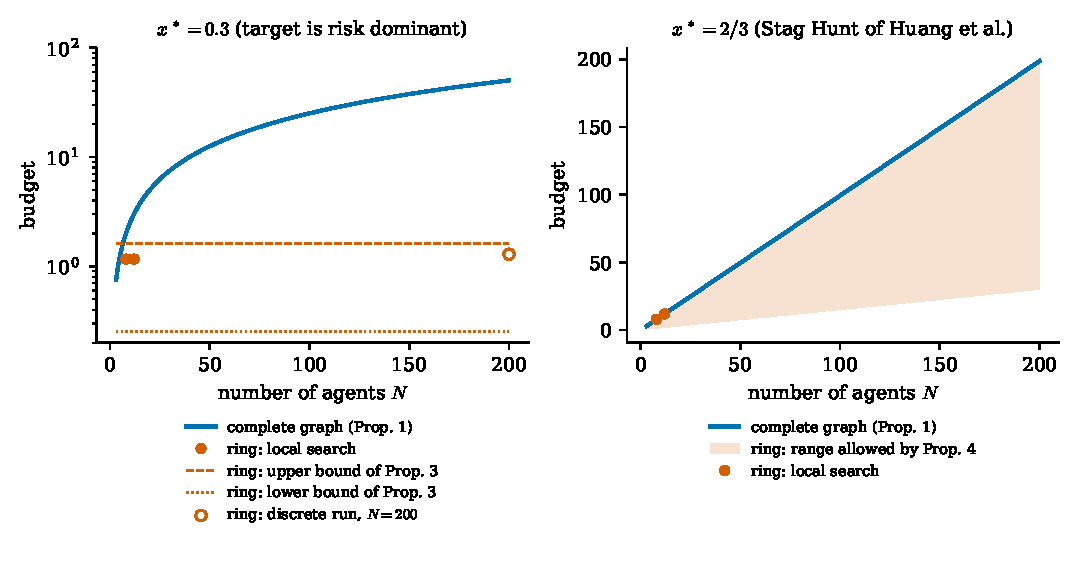
\includegraphics[width=0.98\textwidth]{fig_budget.pdf}
\caption{Smallest budget against the number of agents. Left: $\xs=0.3$, logarithmic vertical axis; the dashed and dotted lines are the two bounds of Proposition~\ref{prop:ring-low} and the open circle is the discrete run of Table~\ref{tab:seed}. Right: $\xs=\tfrac23$, the Stag Hunt of~\cite{huang2025}. The shaded band is the range allowed by Proposition~\ref{prop:ring-high}; Conjecture~\ref{conj:ring-sym} places the ring on its upper edge. In both panels the filled circles are the search of Table~\ref{tab:search} at $N=8$ and $N=12$.}\label{fig:budget}
\end{figure}

\paragraph{Discrete run at $N=200$.}
On a ring of $200$ agents with $\alpha=0.01$ and $U_{\max}=10$, only two adjacent agents were paid (Table~\ref{tab:seed}). After the payments stopped, the unsteered dynamics were integrated until both paid agents were above $2\xs$. From there Proposition~\ref{prop:ring-low} gives convergence to all-$H$. The conversion of the other $198$ agents was not simulated.

\begin{table}[H]
\centering\small
\begin{tabular}{rrrrrr}
\toprule
$\xs$ & Steps paid & Cost paid & Energy rise & Smallest seed & Complete graph\\
\midrule
0.2 & 15 & 0.566 & 0.581 & 0.530 & 23.6\\
0.3 & 24 & 1.290 & 1.297 & 1.222 & 50.3\\
\bottomrule
\end{tabular}
\caption{Steering a ring of $200$ agents by paying two adjacent agents. The energy rise is that of the two paid agents when the payments stop. The cost paid is below it because of the step term of Lemma~\ref{lem:identity}. The smallest seed is the cheapest two-agent seed in continuous time, from the block search. The last column is $N\log\frac{1-x_0}{1-\xs}$.}\label{tab:seed}
\end{table}

\subsection{Front times}\label{sec:fronts}

Figure~\ref{fig:fronts} (left) shows the times $t_j$ of Observation~\ref{obs:front} for a seed of two adjacent agents that is paid once, on a ring of $40$ agents for $\xs=0.2$ and of $26$ agents for $\xs=0.3$. The logits of the two agents are raised $5\%$ more than the smallest amount that reaches the basin. The ratios $t_{j+1}/t_j$ converge to $1.667$ for $\xs=0.2$ and to $2.500$ for $\xs=0.3$; $1/(1-2\xs)$ gives $1.667$ and $2.500$. The differences $K_j=t_{j+1}-\rho t_j$ settle at $1.625$ for $\xs=0.2$ and at $2.948$ for $\xs=0.3$. The agents opposite the seed are left out of these statements, because the front reaches them from both sides. With a decay of $\lambda=0.05$ the times grow linearly. At that $\lambda$ the inferior equilibrium still exists.

\begin{figure}[!ht]
\centering
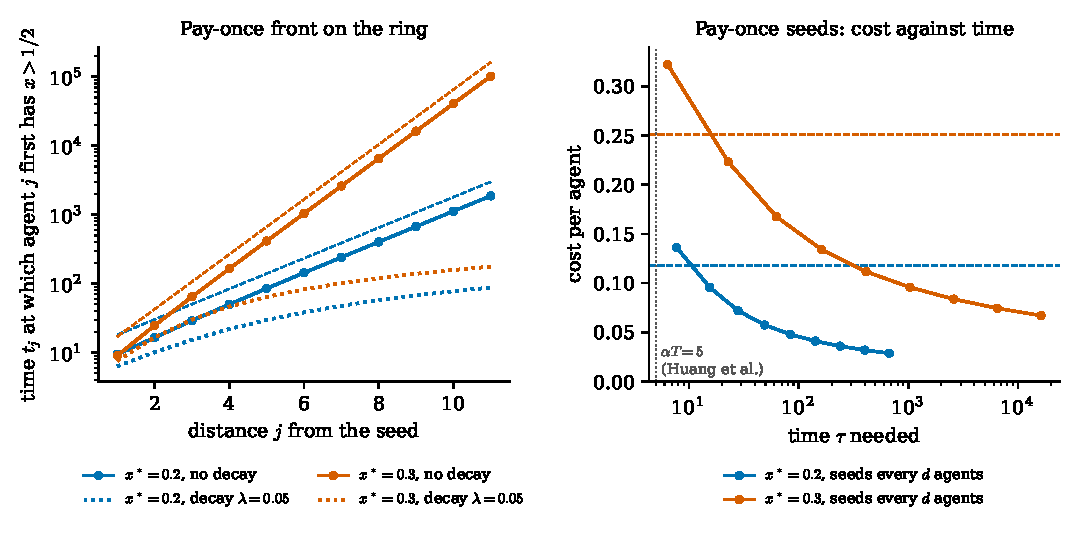
\includegraphics[width=0.98\textwidth]{fig_fronts.pdf}
\caption{Left: time at which the agent at distance $j$ from a pay-once seed first has $x>\tfrac12$. Solid: no decay. Dashed: slope $1/(1-2\xs)$. Dotted: decay $\lambda=0.05$. Right: cost per agent against the time needed, when pay-once seeds are placed every $d$ agents. Horizontal lines: symmetric cost per agent.}\label{fig:fronts}
\end{figure}

Table~\ref{tab:hold} compares a pay-once seed with the strategy of Proposition~\ref{prop:hold} for $\xs=0.3$, with the pair seeded to $y=2\xs+0.02$.

\begin{table}[H]
\centering\small
\begin{tabular}{rlrrr}
\toprule
$N$ & Strategy & Time $\tau$ until all $x>\tfrac12$ & Seed cost & Holding cost\\
\midrule
12 & pay once & 301 & 1.724 & 0\\
16 & pay once & 1903 & 1.724 & 0\\
20 & pay once & 11916 & 1.724 & 0\\
20 & seed and hold & 246 & 1.724 & 0.00001\\
40 & seed and hold & 581 & 1.724 & 0.00008\\
80 & seed and hold & 1252 & 1.724 & 0.00039\\
160 & seed and hold & 2592 & 1.724 & 0.00174\\
\bottomrule
\end{tabular}
\caption{Ring, $\xs=0.3$. Holding payments keep unreached agents at $x_h=10^{-8}$.}\label{tab:hold}
\end{table}

\paragraph{A finite horizon.}
With pay-once seeds every $d$ agents, the cost per agent is the seed cost divided by $d$ and the time is that of a ring of $d$ agents (Figure~\ref{fig:fronts}, right; Table~\ref{tab:cell}). At $\alpha T=5$, the horizon of~\cite{huang2025}, none of these spacings finishes in time. A hop cannot be much faster than the logit distance divided by $c(\tfrac12-\xs)$, which is several time units, so I expect holding payments not to change this.

\begin{table}[H]
\centering\small
\begin{tabular}{rrr}
\toprule
Spacing $d$ & Cost per agent & Time $\tau$ needed\\
\midrule
4 & 0.322 & 6.4\\
6 & 0.223 & 22.8\\
8 & 0.167 & 62.8\\
10 & 0.134 & 162.6\\
12 & 0.112 & 412.1\\
14 & 0.096 & 1035.8\\
16 & 0.084 & 2595.2\\
18 & 0.074 & 6493.6\\
20 & 0.067 & 16239.7\\
\bottomrule
\end{tabular}
\caption{Ring, $\xs=0.3$, pay-once two-agent seeds every $d$ agents. Each seed has a logit shift $5\%$ above the smallest one that reaches the basin on a ring of $d$ agents. The symmetric cost per agent is $0.251$.}\label{tab:cell}
\end{table}

\subsection{Sampled payoffs}\label{sec:feedback}

The identity uses exact payoffs: the learner credits $H$ with the offered payment even in steps where it does not play $H$. In Table~\ref{tab:feedback} one agent, with no game, is moved from $x_0=0.1$ to $\tfrac23$ with an offer of $10$ on $H$ and $\alpha=0.01$, under three feedback models. Moving the exact learner costs slightly less than the energy because of the step term.

\begin{table}[H]
\centering\small
\begin{tabular}{lr}
\toprule
Learner & Cost\\
\midrule
Exact expected advantage (this note) & 0.971\\
Sampled actions, importance-weighted update & 0.900\\
Sampled actions, update only on payments received & 2.900\\
\bottomrule
\end{tabular}
\caption{One agent, three feedback models. The energy is $0.993$ and the logit distance is $2.89$. In the two sampled models the mediator pays $\alpha\times10=0.1$ each time $H$ is played, and the logit moves only then. The number of plays needed is therefore fixed: $9$ with importance weights and $29$ without.}\label{tab:feedback}
\end{table}

For a learner that updates only on payments it receives, the cost is the full logit distance, $\operatorname{logit}\xs-\operatorname{logit}x_0=2.89$. This distance is unbounded as $x_0\to0$. With importance weights a single update has size $\alpha v/x$, which is large when $x$ is small. The large-step effect of Remark~\ref{rem:steps} then appears even for small $\alpha$. The lower bound of Proposition~\ref{prop:complete} does not carry over to this learner.

%=====================================================================
\section{A consistency check with Figure~5 of Huang et al.}\label{sec:bench}

Huang et al.\ train steering strategies with proximal policy optimisation for the two-player Stag Hunt with $\alpha=0.01$, $T=500$ and $U_{\max}=10$. Their training objective is a weight $\beta$ times a goal term minus the cost. A larger $\beta$ buys a smaller gap at a higher cost. Their Figure~5 reports the mean terminal gap and the mean cost for $\beta=10$, $25$ and $100$, over $25$ initial policies on the grid $\{0.1,0.3,0.5,0.7,0.9\}^2$. The largest total utility is $10$, so the gap is $10$ minus the total utility of the policies. The figure is vector graphics. From the coordinates of the bars the values are $3.8$, $2.5$ and $0.6$ ($\times10^{-3}$) for the gap and $5.02$, $6.10$ and $9.03$ for the cost. The $95\%$ error bars are $\pm0.29$, $\pm0.31$ and $\pm0.43$ on the cost and $\pm0.2$, $\pm0.4$ and $\pm0.1$ ($\times10^{-3}$) on the gap.

\paragraph{What the identity predicts.}
Let the agents end at $x_i=1-\delta_i$. By~\eqref{eq:identity-ct} the cost is $\sum_i\log\frac1{\delta_i}$ plus terms that stay bounded as $\delta_i\to0$. For this game the total utility is $4+6x_1x_2$, so the gap is $6(\delta_1+\delta_2)$ to first order. The cost for a target gap $\varepsilon$ is therefore $2\log\frac1\varepsilon$ plus a constant: each halving of the gap costs about $2\log2$.

\paragraph{A reference curve.}
I computed the trade-off between mean terminal gap and mean cost with a threshold rule: pay $U_{\max}$ on $H$ to an agent while its logit is below $K$, and nothing otherwise. Each $K$ gives one point. A dynamic programme on a $201\times201$ grid of logits with $21$ payment levels gives the same curve within $1\%$. An exact programme could not cost more than the rule, because the rule uses only the payments $0$ and $U_{\max}$, which the programme allows. The grid programme costs up to $1\%$ more, so the difference is its grid error. Both are costs of actual strategies, so they are upper bounds on the smallest cost.

\begin{figure}[!ht]
\centering
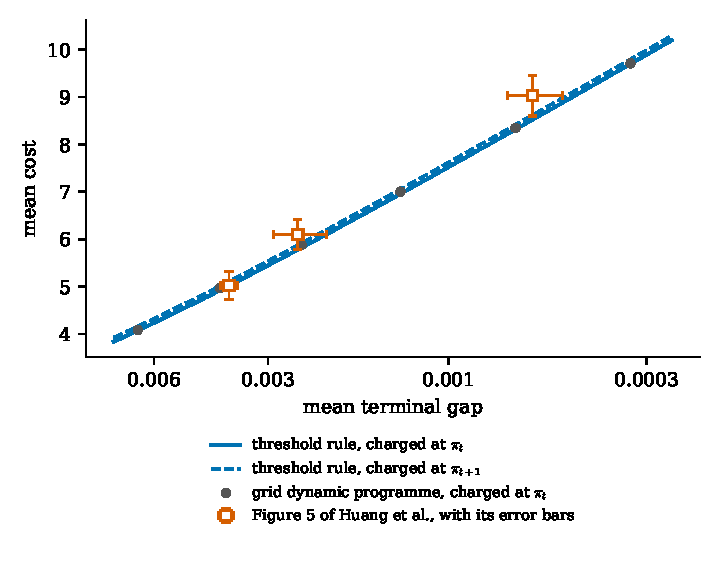
\includegraphics[width=0.62\textwidth]{fig_frontier.pdf}
\caption{Mean cost against mean terminal gap for the two-player Stag Hunt of Huang et al.~\cite{huang2025}. The horizontal axis is logarithmic and decreases to the right. Lines: threshold rule, with the payment charged at $\pi_t$ and at $\pi_{t+1}$. Dots: grid dynamic programme, charged at $\pi_t$. Squares: Figure~5 of~\cite{huang2025}, with its error bars.}\label{fig:frontier}
\end{figure}

\begin{table}[H]
\centering\small
\begin{tabular}{rrrrr}
\toprule
$\beta$ & Reported gap & Reported cost & Rule, charged at $\pi_t$ & Rule, charged at $\pi_{t+1}$\\
\midrule
10 & $3.8\times10^{-3}$ & 5.02 & 5.02 & 5.11\\
25 & $2.5\times10^{-3}$ & 6.10 & 5.78 & 5.87\\
100 & $0.6\times10^{-3}$ & 9.03 & 8.52 & 8.62\\
\bottomrule
\end{tabular}
\caption{Figure~5 of Huang et al.~\cite{huang2025} against the threshold rule at the same gap.}\label{tab:bench}
\end{table}

The slope of the curve is about $1.8$ to $1.9$ per unit of $\log(1/\text{gap})$ in this range, against $2$ in the limit. With the payment charged at $\pi_{t+1}$ the three reported costs are within about $0.4$ of the rule, which is the size of the error bars.

\paragraph{Cautions.}
(i) The released code multiplies each payment by a time interval of $0.01$, and I read the reported costs in these units. In payoff units they would be a hundred times larger. (ii) The released code charges the payment at the updated policy, while the definition in the paper charges it at $\pi_t$. The difference is about $0.1$. (iii) The strategies of~\cite{huang2025} were trained with a goal term in every step (their Eq.~(12)), not on this terminal trade-off. (iv) I did not find the script that produced Figure~5 in the repository.

The check supports one statement. The reported costs lie on or slightly above the cost of a simple threshold rule at the same gap, and they grow with $\log(1/\text{gap})$ at a rate consistent with the $2\log\frac1\varepsilon$ of the identity. The check does not rank the learned strategies.

From the start $(0.1,0.1)$ the rule needs $7.1$, $7.9$ and $10.6$ to reach the three reported gaps, against $1.99$ for entering the basin (Section~\ref{sec:intro}). The difference pays for the rise of the energy of the final policy. The game returns part of that rise after the agents pass $\xs$.

%=====================================================================
\section{Related work}\label{sec:related}

\paragraph{Steering learners with payments.}
Besides the results of~\cite{huang2025} and~\cite{zhang2024} described in the introduction, Huang et al.\ formulate steering as a finite-horizon decision problem over policies and give algorithms for an unknown learning rule. Widmer, Huang and He~\cite{widmer2025} study steering in mean-field games with no-regret agents and an unknown model. Zhang et al.\ steer no-regret learners to an equilibrium with a total payment that grows sublinearly in the horizon. Their impossibility result uses learners that may behave adversarially within the class. Loftin and Oliehoek~\cite{loftin2022} prove a related impossibility for cooperation with every adaptive partner. In both results the obstacle is a partner whose adaptation is unconstrained. The agents of this note follow one known rule. Canyakmaz et al.~\cite{canyakmaz2025} identify unknown game dynamics and steer them with model predictive control. Assos, Dagan and Daskalakis~\cite{assos2024} optimise against a replicator learner (Remark~\ref{rem:origin}). Yang et al.~\cite{yang2020} and Baumann et al.~\cite{baumann2020} let agents or a planner learn to pay learning agents. Ratliff and Fiez~\cite{ratliff2018} and Maheshwari et al.~\cite{maheshwari2022} adapt incentives so that the induced equilibrium is the desired one.

\paragraph{Incentives in evolutionary dynamics and control.}
Riehl, Ramazi and Cao~\cite{riehl2017} and Sakhaei, Maleki and Ramazi~\cite{sakhaei2022} pose the problem closest to this note. They ask for the smallest total reward that drives a network of imitating or best-responding agents to a desired action, with uniform, targeted or budgeted rewards. Their agents switch between pure actions, the reward is a fixed bonus, and the answer is an algorithm. Han and Tran-Thanh~\cite{han2018}, Duong and Han~\cite{duong2021} and Cimpeanu, Han and Santos~\cite{cimpeanu2019} study the cost of institutional incentives in finite and networked populations. Wang et al.~\cite{wang2023} derive optimal incentive protocols with a quadratic running cost under replicator-type dynamics. Their cumulative reward cost contains the term $\ln\frac{1-p_0}{\delta}$, the same logarithm as in Proposition~\ref{prop:complete}. With the linear expected-payment cost of~\cite{huang2025} only the logarithm remains.

\paragraph{Coordination on networks.}
Section~\ref{sec:ring} uses several papers on this topic. Two more are relevant. Raducha and San Miguel~\cite{raducha2022} compare replicator, best-response and imitation updates for coordination games on random graphs. Dall'Asta~\cite{dallasta2021} analyses equilibrium selection in coordination problems on networks.

\paragraph{Where learning converges.}
Mertikopoulos and Sandholm~\cite{mertikopoulos2016} analyse regularised learning in games. Giannou et al.~\cite{giannou2021} show that under follow-the-regularised-leader a Nash equilibrium is stable and attracting with high probability if and only if it is strict. Giannou et al.~\cite{giannou2022} prove local convergence of projected policy gradient in stochastic games. They name methods based on softmax choice, that is exponential weights, as an open question for general stochastic games. Leonardos et al.~\cite{leonardos2022} prove convergence of independent policy gradient in Markov potential games. Bichler, Durmann and Oberlechner~\cite{bichler2024} show that mean-based learners, which include exponential weights, end in the correlated rationalisable set. In a coordination game both actions are rationalisable, so that result does not select an equilibrium. Legacci, Mertikopoulos and Pradelski~\cite{legacci2024} decompose a finite game into a potential part and an incompressible part. Incompressible games are exactly the harmonic games. In them continuous-time exponential weights is Poincar\'e recurrent. Legacci et al.~\cite{legacci2024b} extend this to follow-the-regularised-leader dynamics and show that an extrapolation step restores convergence. Bichler et al.~\cite{bichler2025} relate the size of the potential part to convergence empirically. The game of this note is a potential game. The deterministic limit of learning used here follows~\cite{sato2003,bloembergen2015,barfuss2019}.

\paragraph{Leaders and interventions.}
In the hypergradient method of Grontas et al.~\cite{grontas2024} and in the Stackelberg learning of Maddux et al.~\cite{maddux2025} the followers' game is strongly monotone. Each intervention then has one follower equilibrium, and the leader's cost is a function of the intervention alone. Budget-constrained personalised incentives for traffic routing are designed in the same way~\cite{grontas2023}. In the feedback controllers of Belgioioso et al.~\cite{belgioioso2024} the plant need not be at steady state while the controller acts. That is also the case here. Their closed loop tracks one moving equilibrium, and here the payment moves the learners from one equilibrium to another. The coordination game is a simple game outside the monotone class. Its payoff gradient has Jacobian $c$ times the neighbour-averaging matrix, which has eigenvalue one, so the game is not monotone. It has two strict equilibria, the learners reach one or the other depending on the start, and the payment acts on the path between them. The budget in~\cite{grontas2023} bounds what the authority spends at the followers' equilibrium. The budget here is spent on the way from one equilibrium to the other.

%=====================================================================
\section{Limitations}\label{sec:limits}

\begin{enumerate}
\item \textbf{Exact payoffs.} All results use Assumption~\ref{as:all}. The cost of a unit of logit is $x$ and not $1$ because the learner responds to an offer it does not collect. Table~\ref{tab:feedback} shows how much this matters.
\item \textbf{Small steps.} Propositions~\ref{prop:complete} to~\ref{prop:hold} are for continuous time. In discrete time with the charge at $\pi_t$ the upper bounds hold up to the step term, which is small only when $\alpha U_{\max}\ll1$ (Table~\ref{tab:steps}). The lower bounds of Propositions~\ref{prop:ring-low} and~\ref{prop:ring-high} carry over to discrete time with the factor $\alpha U_{\max}/(e^{\alpha U_{\max}}-1)$, which is $0.95$ at the parameters of~\cite{huang2025}. The reason is that a step with $g_i\le0$ raises the energy by at most $x_i(e^{\alpha v_i}-1)$, and its cost is $\alpha x_iv_i$. For Proposition~\ref{prop:complete} I have no such bound, because single agents can have $g_i>0$ before the average reaches $\xs$. There the discrete statement rests on Table~\ref{tab:steps}.
\item \textbf{Local search.} Conjectures~\ref{conj:ring-sym} and~\ref{conj:seed} rest on a local search at $N=8$ and $N=12$, on strategies that pay once. A cheaper state that the search missed, or a strategy that pays in several stages, would refute them. The proved bounds do not depend on the search.
\item \textbf{Observations.} Observations~\ref{obs:front} and~\ref{obs:decay} are numerical, for two values of $\xs$. Observation~\ref{obs:front} holds for pay-once strategies only.
\item \textbf{Two graphs.} I have no result for lattices, random graphs or networks with hubs. The contagion threshold of a graph can be anywhere up to $\tfrac12$~\cite{morris2000}. I expect a bounded budget below a graph-dependent threshold, and have not checked it.
\item \textbf{Common start and common game.} All agents start at the same $x_0$ and play the same game.
\item \textbf{No noise.} For $\xs>\tfrac12$, as in the Stag Hunt of~\cite{huang2025}, $G$ is risk dominant. For a learner with logit noise, all-$G$ is then the stochastically stable state (Section~\ref{sec:ring}), so a population steered to all-$H$ would leave it again after a long time. The budget then keeps the population at all-$H$ for a long but finite time. With the exact rule the change is permanent.
\item \textbf{Non-negative rewards.} The budget exists because steering rewards are non-negative, as in~\cite{huang2025}. A mediator who could tax action $G$ would move the same learners at a profit.
\item \textbf{The check of Section~\ref{sec:bench}} depends on my reading of the released code and of the published figure.
\item \textbf{Brackets.} On the ring the smallest budget is only bracketed. At $\xs=0.3$ the bounds are $0.251$ and $1.62$.
\item \textbf{Two actions.} All results are for two actions. Remark~\ref{rem:other} gives only the identity for more.
\end{enumerate}

%=====================================================================
\section{Open questions}\label{sec:next}

\begin{enumerate}
\item \textbf{A cap and a horizon.} With the identity, and payments on $H$ only, minimising the cost for fixed end points is the same as maximising $\int\sum_ix_ig_i\,d\tau$. For two players the threshold rule of Section~\ref{sec:bench} costs within $1\%$ of a dynamic programme on a grid. Is the threshold rule optimal?
\item \textbf{Budget against waiting time.} When $\xs<\tfrac12$, logit noise selects all-$H$ on every network (Section~\ref{sec:ring}). Payment is then not needed for the outcome. It only shortens the waiting time. Theorem~3.1 of Maddux et al.~\cite{maddux2024} bounds the waiting time for games with $A\ge4$ actions. The game here has two actions, which is outside that assumption. The bound grows like $(A^N/\epsilon)^{1/\Delta}$, where $\Delta$ is the gap between the two best values of the potential scaled to $[0,1]$. On the ring one deviator from all-$H$ changes the scaled potential by about $2/N$, so $\Delta$ is of order $1/N$. The steering budget is bounded on the ring and linear on the complete graph. How much budget replaces how much waiting?
\item \textbf{Bandit feedback.} What is the smallest expected budget for importance-weighted learners~\cite{mertikopoulos2023,fiegel2025}? Table~\ref{tab:feedback} shows that the answer differs from the exact case. In that one example the large updates of the importance-weighted estimator lower the cost. In~\cite{fiegel2025} this estimator is used without an implicit-exploration correction, and the regularisation towards the uniform policy is what gives last-iterate convergence.
\item \textbf{Games that are not potential games.} The energy term does not depend on the game. The regret term does. In a harmonic game with strategic centre $(\mu,q)$ in the sense of Legacci et al.~\cite{legacci2024b}, with weights $\mu_i$ and payoff vectors $w_i(x)$, $\sum_i\mu_i\langle w_i(x),x_i-q_i\rangle=0$ for every $x$ (their Proposition~A.4). The identity with base point $q$ then reads $\sum_i\mu_i\int\langle u_i,x_i-q_i\rangle\,d\tau=\Delta F_{\mu,q}$, where $F_{\mu,q}$ is their constant of motion (Proposition~C.1). This is the computation~(C.5) in the proof of that proposition with the steering reward added to the payoff vector. A run in Matching Pennies agrees. The game term of the identity is zero, and without payments the level of $F_{\mu,q}$ is kept. What does a mediator pay to hold a profile there?
\item \textbf{Bilevel methods when the lower level has two equilibria.} Hypergradient methods~\cite{grontas2024} optimise an intervention through the followers' equilibrium map. With two equilibria that map has two branches. The identity gives the cost of moving the learners from one branch to the other as an energy difference plus a regret integral. Can it serve as a switching cost in the upper-level objective?
\item \textbf{General graphs.} Is the budget bounded exactly below the contagion threshold of the graph? On which graphs does a two-coordinate invariance check, as on the ring, replace a check in $N$ dimensions~\cite{czechowski2023}?
\end{enumerate}

%=====================================================================
\appendix
\section{Proofs}\label{app:proofs}

\subsection{Lemma~\ref{lem:one}}
The dynamics depend on the payments only through $v_i$. Subtracting $\min(u_i(H),u_i(G))\ge0$ from both payments lowers the cost and leaves $v_i$ unchanged. If $v_i\ge0$ the reduced cost is $x_iv_i$. If $v_i<0$ it is $(1-x_i)|v_i|\ge0>x_iv_i$. \qed

\subsection{Lemma~\ref{lem:identity}}
Drop the index $i$ and let $\theta'=\theta+s$. Since $1-x=1/(1+e^\theta)$,
\[
1-x'=\frac{1-x}{1-x+xe^{s}},\qquad
E(\theta')-E(\theta)=\log(1-x+xe^{s})=xs+\bigl[\log(1-x+xe^{s})-xs\bigr].
\]
The bracket is $\KL(\pi\|\pi')$: indeed $\KL(\pi\|\pi')=x\log\frac{x}{x'}+(1-x)\log\frac{1-x}{1-x'}$, and $\frac{x}{x'}=(1-x+xe^{s})e^{-s}$, $\frac{1-x}{1-x'}=1-x+xe^{s}$. With $xs=\alpha xg+\alpha xv$ this gives~\eqref{eq:identity}. The bracket is non-negative by Jensen's inequality and at most $s^2/8$ by Hoeffding's lemma for a variable that equals $s$ with probability $x$ and $0$ otherwise. The algebra holds for either sign of $v$, and by Lemma~\ref{lem:one} the step cost is at least $\alpha xv$. In continuous time $\frac{d}{d\tau}E(\theta)=x\dot\theta=x(g+v)$. \qed

\subsection{Proposition~\ref{prop:complete}}
\emph{Lower bound.} Let $S=\sum_ix_i$ and $\bar x=S/N$. On the complete graph $m_i=(S-x_i)/(N-1)$, so
\[
\sum_ix_im_i=\frac{S^2-\sum_ix_i^2}{N-1}\le\frac{S^2-S^2/N}{N-1}=\frac{S^2}{N},
\qquad
\sum_ix_ig_i\le c\,S\,(\bar x-\xs).
\]
So the total regret term $\sum_ix_i(-g_i)$ is non-negative whenever $\bar x\le\xs$. At the start $\bar x=x_0<\xs$, and a successful strategy ends with $\bar x\to1$. The logits are continuous, so there is a first time $\tau_1$ with $\bar x(\tau_1)=\xs$. Summing Lemma~\ref{lem:identity} over agents on $[0,\tau_1]$,
\[
\text{cost up to }\tau_1\;\ge\;\En(\theta(\tau_1))-\En(\theta(0))=\sum_i\bigl(-\log(1-x_i(\tau_1))\bigr)+N\log(1-x_0).
\]
The function $-\log(1-x)$ is convex, so $\sum_i-\log(1-x_i(\tau_1))\ge-N\log(1-\xs)$. Costs after $\tau_1$ are non-negative.

\emph{Upper bound.} Use the strategy of Proposition~\ref{prop:cap} with target $\xs+\epsilon$. When it stops, every $m_i=\xs+\epsilon>\xs$ and every logit increases. This condition is preserved when all $x_i$ increase, so all $x_i\to1$. The cost tends to $N\log\frac{1-x_0}{1-\xs-\epsilon}$ as $U\to\infty$. \qed

The same argument proves Remark~\ref{rem:general}: it uses only that the total regret term is non-negative while $W\le0$, and on the graphs named there $\sum_ix_im_i\le S^2/N$. For the ring with four agents, $\sum_ix_im_i=(x_1+x_3)(x_2+x_4)\le S^2/4$.

\subsection{Proposition~\ref{prop:cap}}
In a symmetric state $m_i=x$ on any graph, so every agent follows $\dot\theta=U+c(x-\xs)>0$ on $[x_0,\xs]$. The cost rate per agent is $xU$. With $d\theta=dx/(x(1-x))$ and $a=U-c\xs$,
\[
\frac{C_{\mathrm{sym}}}{N}=\int_{x_0}^{\xs}\frac{U\,dx}{(a+cx)(1-x)}=\frac{U}{a+c}\log\frac{(a+c\xs)(1-x_0)}{(a+cx_0)(1-\xs)},
\]
by $\frac{1}{(a+cx)(1-x)}=\frac{1}{a+c}\bigl(\frac{c}{a+cx}+\frac{1}{1-x}\bigr)$. This is~\eqref{eq:cap}. The time is $\int_{x_0}^{\xs}\frac{dx}{x(1-x)(a+cx)}$, and partial fractions give~\eqref{eq:captime}. The integrand of the cost decreases in $U$ for every $x<\xs$. \qed

\subsection{Proposition~\ref{prop:ring-low}}
\emph{Lower bound, any graph.} Let $\tau_1$ be the first time at which some agent $i$ reaches $\xs$. It exists for a successful strategy. Before $\tau_1$ every $x_j<\xs$, so $m_i<\xs$ and $g_i<0$. The regret term of agent $i$ is non-negative on $[0,\tau_1]$, and by Lemma~\ref{lem:identity} its cost is at least $E(\theta_i(\tau_1))-E(\theta_i(0))=\log\frac{1-x_0}{1-\xs}$.

\emph{Upper bound.} Pay two adjacent agents $a$ and $b$ at a large constant rate until both have $x=y$, where $2\xs<y<1$. By~\eqref{eq:identity-ct} the cost of each is $\log\frac{1-x_0}{1-y}$ plus its regret term, which is at most $c$ times the duration of the payment and tends to zero with it. Now stop paying. Agent $a$ has neighbours $b$ and one other agent, so $m_a\ge x_b/2\ge y/2>\xs$, and the same holds for $b$. Suppose one of them later has a neighbour average of at most $\xs$, and let $\tau'$ be the first such time. Before $\tau'$ both logits were increasing, so $x_a,x_b\ge y$ at $\tau'$ and both averages are at least $y/2>\xs$. This is a contradiction. So $x_a$ and $x_b$ increase for ever.

The other neighbour of $a$ has $m\ge x_a/2\ge y/2$, so its logit rises at rate at least $c(y/2-\xs)>0$ and reaches $y$ in finite time. It then forms an adjacent pair above $y$ with $a$, and the argument repeats. By induction every agent reaches $y$. Then every $m_i\ge y>\xs$ and all $x_i\to1$. Letting $y\downarrow2\xs$ gives the bound. \qed

\subsection{Proposition~\ref{prop:ring-high}}
\emph{Upper bound.} The symmetric strategy works on any graph.

\emph{Lower bound.} Let $z=2\xs-1$. By assumption $x_0<z<1$. For a successful strategy every agent reaches $z$; let $\sigma_i$ be the first time agent $i$ does. Call agent $i$ \emph{helped} if both its neighbours reach $z$ strictly before $\sigma_i$. Two adjacent agents cannot both be helped, because each would have to reach $z$ strictly before the other. So at most $\lfloor N/2\rfloor$ agents are helped. Let $i$ be an agent that is not helped. It has a neighbour $j$ with $x_j\le z$ on $[0,\sigma_i]$. Then $m_i\le\frac12(z+1)=\xs$ on $[0,\sigma_i]$, so $g_i\le0$ and the regret term of agent $i$ is non-negative there. By Lemma~\ref{lem:identity} the cost of agent $i$ is at least $E(\theta_i(\sigma_i))-E(\theta_i(0))=\log\frac{1-x_0}{1-z}=\log\frac{1-x_0}{2(1-\xs)}$. There are at least $\lceil N/2\rceil$ such agents. \qed

\subsection{Proposition~\ref{prop:hold}}
Seed the pair $a,b$ to $y$ as in Proposition~\ref{prop:ring-low}, at a cost that tends to $2\log\frac{1-x_0}{1-y}$. Fix $x_h\in(0,x_0)$ and $\theta_h=\operatorname{logit}x_h$. For every other agent $i$: whenever $\theta_i=\theta_h$ and $g_i<0$, pay $v_i=-g_i$ on $H$; otherwise pay nothing. Then $\dot\theta_i\ge0$ at $\theta_h$, so $\theta_i\ge\theta_h$ at all times. Payments are non-negative, so the argument of Proposition~\ref{prop:ring-low} still shows that the block of agents above $y$ never shrinks and that the agent next to it has $g\ge r=c(y/2-\xs)$. That agent starts at or above $\theta_h$ and reaches $y$ within a time $(\operatorname{logit}y-\theta_h)/r\le(\operatorname{logit}y+\log\frac{1}{x_h})/r$. There are two fronts and at most $N/2$ hops, so all agents are above $y$ after a time
\[
\tau_N\le\frac{N}{2r}\Bigl(\operatorname{logit}y+\log\frac1{x_h}\Bigr),
\]
and the strategy stops there. A held agent has $x=x_h$ and $|g|\le c\,\xs$, so the holding cost is at most $N\,x_h\,c\,\xs\,\tau_N$. With $x_h=\epsilon'/N^{3}$ this is of order $\epsilon'\log(N/\epsilon')/N$, which is below $\epsilon$ for $\epsilon'$ small, and $\tau_N$ is of order $\frac Nr\log\frac N\epsilon$. \qed

\section{Code}\label{app:code}

The code and the result files are at \texttt{\codeurl}. The code needs Python with NumPy, Numba and Matplotlib. \texttt{verify\_note.py} also needs SciPy.

\begin{center}\small
\begin{tabular}{p{0.3\textwidth}p{0.6\textwidth}}
\toprule
File & Content\\
\midrule
\texttt{steer.py} & Dynamics, basin test, steering simulation, local search, closed form\\
\texttt{run\_checks.py} & Table~\ref{tab:cap}; a numerical check of Lemma~\ref{lem:identity}\\
\texttt{run\_search.py}, \texttt{run\_refine.py} & Table~\ref{tab:search}; the block search\\
\texttt{run\_fronts.py} & Tables~\ref{tab:seed} and~\ref{tab:cell}, the front times of Figure~\ref{fig:fronts}\\
\texttt{run\_extra.py} & Tables~\ref{tab:steps}, \ref{tab:hold} and~\ref{tab:feedback}; the Euclidean and harmonic checks\\
\texttt{threshold\_rule.py}, \texttt{frontier\_dp.py}, \texttt{bench\_dp.py} & Section~\ref{sec:bench}\\
\texttt{make\_figs.py} & Figures~\ref{fig:budget} to~\ref{fig:frontier}\\
\texttt{fill\_tables.py} & Writes the numbers of the eight tables into the source of this note\\
\texttt{verify\_note.py} & Independent numerical checks of the lemmas, the closed forms and the numbers quoted in the text\\
\bottomrule
\end{tabular}
\end{center}

The basin test integrates the unsteered dynamics and stops when all neighbour averages are above $\xs$ (the state then converges to all-$H$) or all are below (all-$G$). These rules are exact because the dynamics preserve the componentwise order of states. On the ring the test also stops by the invariant boxes of Propositions~\ref{prop:ring-low} and~\ref{prop:ring-high}. So the code cannot be used to test those two propositions. All continuous-time runs use a classical Runge--Kutta step: $0.05$ for the basin test and the front times, and $0.02$ for the runs with holding payments. In Table~\ref{tab:search} the rows with $\xs<\tfrac12$ are the output of \texttt{run\_refine.py}, which optimises blocks of two to five adjacent agents. The rows with $\xs>\tfrac12$ are the output of \texttt{run\_search.py}.

\begin{thebibliography}{99}\small
\setlength{\itemsep}{0.15em}

\bibitem{huang2025} J.~Huang, V.~Thoma, Z.~Shen, H.~H.~Nax, N.~He. Learning to steer Markovian agents under model uncertainty. \emph{ICLR}, 2025. arXiv:2407.10207.
\bibitem{zhang2024} B.~H.~Zhang, G.~Farina, I.~Anagnostides, F.~Cacciamani, S.~McAleer, A.~Haupt, A.~Celli, N.~Gatti, V.~Conitzer, T.~Sandholm. Steering no-regret learners to a desired equilibrium. \emph{EC}, 2024. arXiv:2306.05221.
\bibitem{widmer2025} L.~Widmer, J.~Huang, N.~He. Steering no-regret agents in MFGs under model uncertainty. \emph{AISTATS}, 2025. arXiv:2503.09309.
\bibitem{canyakmaz2025} I.~Canyakmaz, I.~Sakos, W.~Lin, A.~Varvitsiotis, G.~Piliouras. Learning and steering game dynamics towards desirable outcomes. 2024. arXiv:2404.01066.
\bibitem{assos2024} A.~Assos, Y.~Dagan, C.~Daskalakis. Maximizing utility in multi-agent environments by anticipating the behavior of other learners. 2024. arXiv:2407.04889.
\bibitem{monderer2004} D.~Monderer, M.~Tennenholtz. K-implementation. \emph{JAIR}, 2004. arXiv:1107.0022.
\bibitem{mertikopoulos2016} P.~Mertikopoulos, W.~H.~Sandholm. Learning in games via reinforcement and regularization. \emph{Mathematics of Operations Research}, 2016. arXiv:1407.6267.
\bibitem{kwon2017} J.~Kwon, P.~Mertikopoulos. A continuous-time approach to online optimization. \emph{Journal of Dynamics and Games}, 2017. arXiv:1401.6956.
\bibitem{sorin2020} S.~Sorin. Replicator dynamics: old and new. \emph{Journal of Dynamics and Games}, 2020.
\bibitem{derooij2014} S.~de Rooij, T.~van Erven, P.~D.~Gr\"unwald, W.~M.~Koolen. Follow the leader if you can, hedge if you must. \emph{JMLR}, 2014. arXiv:1301.0534.
\bibitem{legacci2024b} D.~Legacci, P.~Mertikopoulos, C.~H.~Papadimitriou, G.~Piliouras, B.~S.~R.~Pradelski. No-regret learning in harmonic games: extrapolation in the face of conflicting interests. \emph{NeurIPS}, 2024. arXiv:2412.20203.
\bibitem{legacci2024} D.~Legacci, P.~Mertikopoulos, B.~Pradelski. A geometric decomposition of finite games: convergence vs.\ recurrence under exponential weights. \emph{ICML}, 2024. arXiv:2405.07224.
\bibitem{giannou2021} A.~Giannou, E.-V.~Vlatakis-Gkaragkounis, P.~Mertikopoulos. Survival of the strictest: stable and unstable equilibria under regularized learning with partial information. \emph{COLT}, 2021. arXiv:2101.04667.
\bibitem{mertikopoulos2023} P.~Mertikopoulos, Y.-P.~Hsieh, V.~Cevher. A unified stochastic approximation framework for learning in games. \emph{Mathematical Programming}, 2023. arXiv:2206.03922.
\bibitem{giannou2022} A.~Giannou, K.~Lotidis, P.~Mertikopoulos, E.-V.~Vlatakis-Gkaragkounis. On the convergence of policy gradient methods to Nash equilibria in general stochastic games. \emph{NeurIPS}, 2022. arXiv:2210.08857.
\bibitem{kakade2001} S.~Kakade. A natural policy gradient. \emph{NeurIPS}, 2001.
\bibitem{agarwal2021} A.~Agarwal, S.~M.~Kakade, J.~D.~Lee, G.~Mahajan. On the theory of policy gradient methods: optimality, approximation, and distribution shift. \emph{JMLR}, 2021. arXiv:1908.00261.
\bibitem{alatur2024} P.~Alatur, A.~Barakat, N.~He. Independent policy mirror descent for Markov potential games: scaling to large number of players. \emph{IEEE Conference on Decision and Control}, 2024. arXiv:2408.08075.
\bibitem{cayci2021} S.~Cayci, N.~He, R.~Srikant. Convergence of entropy-regularized natural policy gradient with linear function approximation. \emph{SIAM Journal on Optimization}, 2024. arXiv:2106.04096.
\bibitem{gao2018} B.~Gao, L.~Pavel. On passivity, reinforcement learning and higher-order learning in multi-agent finite games. \emph{IEEE Transactions on Automatic Control}, 2021. arXiv:1808.04464.
\bibitem{leonardos2022} S.~Leonardos, W.~Overman, I.~Panageas, G.~Piliouras. Global convergence of multi-agent policy gradient in Markov potential games. \emph{ICLR}, 2022. arXiv:2106.01969.
\bibitem{sato2003} Y.~Sato, J.~P.~Crutchfield. Coupled replicator equations for the dynamics of learning in multiagent systems. \emph{Physical Review E}, 2003. arXiv:nlin/0204057.
\bibitem{kianercy2012} A.~Kianercy, A.~Galstyan. Dynamics of Boltzmann Q-learning in two-player two-action games. \emph{Physical Review E}, 2012. arXiv:1109.1528.
\bibitem{bloembergen2015} D.~Bloembergen, K.~Tuyls, D.~Hennes, M.~Kaisers. Evolutionary dynamics of multi-agent learning: a survey. \emph{JAIR}, 2015.
\bibitem{barfuss2019} W.~Barfuss, J.~F.~Donges, J.~Kurths. Deterministic limit of temporal difference reinforcement learning for stochastic games. \emph{Physical Review E}, 2019. arXiv:1809.07225.
\bibitem{morris2000} S.~Morris. Contagion. \emph{Review of Economic Studies}, 2000. Working paper version, CARESS 97-01, University of Pennsylvania.
\bibitem{montanari2009} A.~Montanari, A.~Saberi. Convergence to equilibrium in local interaction games and Ising models. 2008. arXiv:0812.0198.
\bibitem{naxnewton2022} H.~H.~Nax, J.~Newton. Deep and shallow thinking in the long run. \emph{Theoretical Economics}, 2022.
\bibitem{maddux2024} A.~Maddux, R.~Ouhamma, H.~Catic, M.~Kamgarpour. Finite-time convergence to an $\epsilon$-efficient Nash equilibrium in potential games. 2024; version~4, January 2026. arXiv:2405.15497.
\bibitem{cordasco2018} G.~Cordasco, L.~Gargano, J.~G.~Peters, A.~A.~Rescigno, U.~Vaccaro. Time-bounded influence diffusion with incentives. 2018. arXiv:1807.06921.
\bibitem{heijmans2023} R.~J.~R.~K.~Heijmans. Unraveling coordination problems. 2023. arXiv:2307.08557.
\bibitem{sakovics2012} J.~S\'akovics, J.~Steiner. Who matters in coordination problems? \emph{American Economic Review}, 2012. Authors' version.
\bibitem{madeo2015} D.~Madeo, C.~Mocenni. A new mathematical model for evolutionary games on finite networks of players. 2013. arXiv:1307.1670.
\bibitem{raducha2022} T.~Raducha, M.~San Miguel. Coordination and equilibrium selection in games: the role of local effects. \emph{Scientific Reports}, 2022. arXiv:2110.10036.
\bibitem{dallasta2021} L.~Dall'Asta. Coordination problems on networks revisited: statics and dynamics. 2021. arXiv:2106.02548.
\bibitem{riehl2017} J.~Riehl, P.~Ramazi, M.~Cao. Control of asynchronous imitation dynamics on networks. 2017. arXiv:1704.04416.
\bibitem{sakhaei2022} N.~Sakhaei, Z.~Maleki, P.~Ramazi. Equilibration analysis and control of coordinating decision-making populations. 2022. arXiv:2201.04185.
\bibitem{han2018} T.~A.~Han, L.~Tran-Thanh. Cost-effective external interference for promoting the evolution of cooperation. \emph{Scientific Reports}, 2018.
\bibitem{duong2021} M.~H.~Duong, T.~A.~Han. Cost efficiency of institutional incentives for promoting cooperation in finite populations. \emph{Proceedings of the Royal Society A}, 2021. arXiv:2103.01131.
\bibitem{cimpeanu2019} T.~Cimpeanu, T.~A.~Han, F.~C.~Santos. Exogenous rewards for promoting cooperation in scale-free networks. 2019. arXiv:1905.04964.
\bibitem{wang2023} S.~Wang, X.~Chen, Z.~Xiao, A.~Szolnoki, V.~V.~Vasconcelos. Optimization of institutional incentives for cooperation in structured populations. \emph{Journal of the Royal Society Interface}, 2023. arXiv:2301.06472.
\bibitem{panageas2023} I.~Panageas, N.~Patris, S.~Skoulakis, V.~Cevher. Exponential lower bounds for fictitious play in potential games. \emph{NeurIPS}, 2023. arXiv:2310.02387.
\bibitem{fiegel2025} C.~Fiegel, P.~M\'enard, T.~Kozuno, M.~Valko, V.~Perchet. The harder path: last iterate convergence for uncoupled learning in zero-sum games with bandit feedback. \emph{ICML}, 2025. arXiv:2604.16087.
\bibitem{bichler2025b} M.~Bichler, J.~Durmann, M.~Oberlechner. Agentic markets: game dynamics and equilibrium in markets with learning agents. 2025. arXiv:2506.18571.
\bibitem{bichler2024} M.~Bichler, J.~Durmann, M.~Oberlechner. Online optimization algorithms in repeated price competition: equilibrium learning and algorithmic collusion. 2024. arXiv:2412.15707.
\bibitem{bichler2025} M.~Bichler, D.~Legacci, P.~Mertikopoulos, M.~Oberlechner, B.~Pradelski. Characterizing the convergence of game dynamics via potentialness. \emph{Transactions on Machine Learning Research}, 2025. arXiv:2503.16285.
\bibitem{czechowski2023} A.~Czechowski, F.~A.~Oliehoek. Safe multi-agent learning via trapping regions. \emph{IJCAI}, 2023. arXiv:2302.13844.
\bibitem{loftin2022} R.~Loftin, F.~A.~Oliehoek. On the impossibility of learning to cooperate with adaptive partner strategies in repeated games. \emph{ICML}, 2022. arXiv:2206.10614.
\bibitem{grontas2024} P.~D.~Grontas, G.~Belgioioso, C.~Cenedese, M.~Fochesato, J.~Lygeros, F.~D\"orfler. BIG Hype: best intervention in games via distributed hypergradient descent. \emph{IEEE Transactions on Automatic Control}, 2024. arXiv:2303.01101.
\bibitem{grontas2023} P.~D.~Grontas, C.~Cenedese, M.~Fochesato, G.~Belgioioso, J.~Lygeros, F.~D\"orfler. Designing optimal personalized incentive for traffic routing using BIG Hype algorithm. \emph{IEEE Conference on Decision and Control}, 2023. arXiv:2304.12004.
\bibitem{belgioioso2024} G.~Belgioioso, D.~Liao-McPherson, M.~Hudoba de Badyn, S.~Bolognani, R.~S.~Smith, J.~Lygeros, F.~D\"orfler. Online feedback equilibrium seeking. \emph{IEEE Transactions on Automatic Control}, 2025. arXiv:2210.12088.
\bibitem{maddux2025} A.~Maddux, M.~Maljkovic, N.~Geroliminis, M.~Kamgarpour. No-regret learning in Stackelberg games with an application to electric ride-hailing. \emph{IEEE Conference on Decision and Control}, 2025. arXiv:2504.03745.
\bibitem{yang2020} J.~Yang, A.~Li, M.~Farajtabar, P.~Sunehag, E.~Hughes, H.~Zha. Learning to incentivize other learning agents. \emph{NeurIPS}, 2020. arXiv:2006.06051.
\bibitem{baumann2020} T.~Baumann, T.~Graepel, J.~Shawe-Taylor. Adaptive mechanism design: learning to promote cooperation. 2019. arXiv:1806.04067.
\bibitem{ratliff2018} L.~J.~Ratliff, T.~Fiez. Adaptive incentive design. 2018. arXiv:1806.05749.
\bibitem{maheshwari2022} C.~Maheshwari, K.~Kulkarni, M.~Wu, S.~S.~Sastry. Inducing social optimality in games via adaptive incentive design. 2022. arXiv:2204.05507.
\bibitem{maiti2026} A.~Maiti. Attractor count in collective reinforcement-learning dynamics depends on interaction structure, not on population size. Technical report with code, not peer reviewed. Zenodo, version 1.0.1, October 2026. doi:10.5281/zenodo.23264321.
\bibitem{anagnostides2026} I.~Anagnostides, I.~Panageas, N.~Patris, T.~Sandholm. (Doubly) exponential lower bounds for follow the regularized leader in potential games. 2026. arXiv:2601.23248.
\bibitem{cai2024} Y.~Cai, G.~Farina, J.~Grand-Cl\'ement, C.~Kroer, C.-W.~Lee, H.~Luo, W.~Zheng. Fast last-iterate convergence of learning in games requires forgetful algorithms. \emph{NeurIPS}, 2024. arXiv:2406.10631.
\bibitem{su2026} Y.~Su, E.-V.~Vlatakis-Gkaragkounis. No coin left behind: maximizing strategic surplus against no-regret dynamics. 2026. arXiv:2604.05129.
\bibitem{pradelski2012} B.~S.~R.~Pradelski, H.~P.~Young. Learning efficient Nash equilibria in distributed systems. \emph{Games and Economic Behavior}, 2012. Working paper version, Discussion Paper 480, Department of Economics, University of Oxford.
\bibitem{mertikopoulos2026} P.~Mertikopoulos. Regret, equilibrium, and learning in games: a guided tour. 2026. arXiv:2608.09389.
\end{thebibliography}

\end{document}
